% -*- LaTeX -*-
% -*- coding: utf-8 -*-
%
% ~~~~~~~~~~~~~~~~~~~~~~~~~~~~~~~~~~~~~~~~~~~~~~~~~~~~~~~~~~~~~~~~~~~~~~~~~~~~~~
%
%                             michael a.g. aïvázis
%                      california institute of technology
%                      (c) 1998-2010  all rights reserved
%
% ~~~~~~~~~~~~~~~~~~~~~~~~~~~~~~~~~~~~~~~~~~~~~~~~~~~~~~~~~~~~~~~~~~~~~~~~~~~~~~
%

\lecture{Overview}{20100208}

% --------------------------------------
% Overview
\begin{frame}[fragile]
%
  \frametitle{Overview}
%
  \begin{itemize}
%
  \item lattices: logically Cartesian grids
    \begin{itemize}
    \item flow, lattice dynamics, wave propagation, image processing
    \end{itemize}
%
  \item suitable when it is possible to find an invertible map $\phi$ from the problem domain
    $\Omega$ to $\mathbb{Z}^{d}$
%
  \item data representation: multi-dimensional arrays
    \begin{itemize}
    \item $\phi$ maps points in $\Omega$ to loop indices
    \item with {\em guard cells} for enforcing boundary conditions
    \end{itemize}
% 
  \end{itemize}
%
  \begin{figure}
    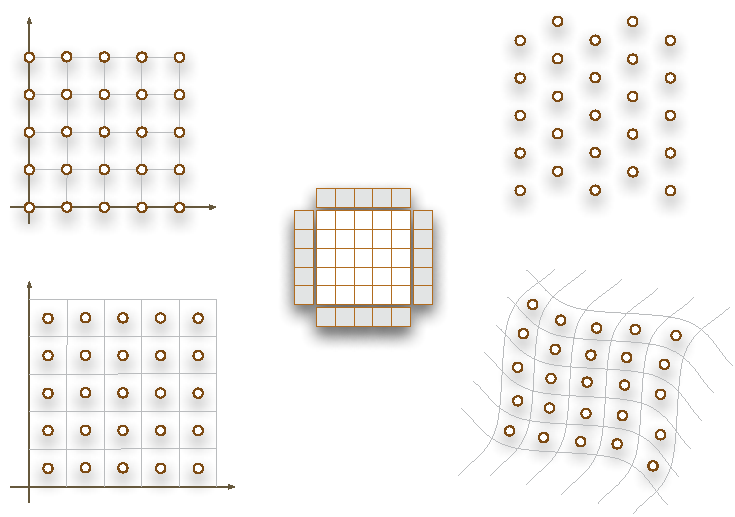
\includegraphics[scale=0.5]{figures/structured.pdf}
  \end{figure} 
%
\end{frame}

% --------------------------------------
% advantages
\begin{frame}[fragile]
%
  \frametitle{Advantages}
%
  \begin{itemize}
%
  \item advantages: logically rectangular
    \begin{itemize}
    \item indexing: easy traversal using loops
    \item fixed stride: predictable memory layout
    \item topology: finding neighbors is trivial
    \end{itemize}
%
    \item disadvantages:
      \begin{itemize}
      \item non-trivial geometries are hard to model
      \end{itemize}
% 
  \end{itemize}
%
\end{frame}

% --------------------------------------
% data layout
\begin{frame}[fragile]
%
  \frametitle{Data layouts}
%
  \begin{itemize}
%
  \item na\"ive use of multi-dimensional arrays does not perform well
    \begin{itemize}
    \item for large problem sizes
    \item for complex physics updates that require keeping track of multiple fields
    \end{itemize}
%
  \item representing scalar, vector and tensor fields
    \begin{itemize}
    \item optimal layout is problem dependent
    \item goal is to minimize cache misses while updating the fields
    \end{itemize}
%
  \item the conventional mapping to arrays lays out the data in matrix form
    \begin{itemize}
    \item not necessarily the most convenient convention
    \end{itemize}
% 
  \end{itemize}
%
  \begin{figure}
    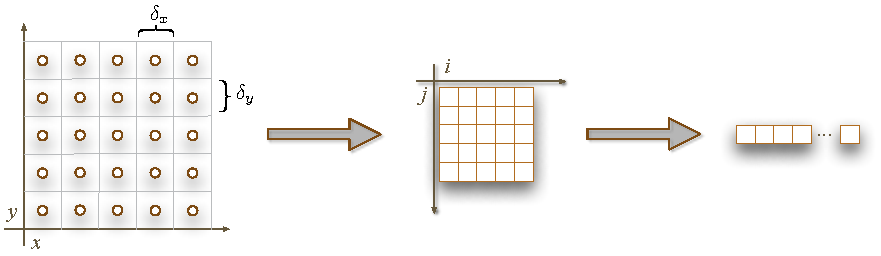
\includegraphics[scale=0.7]{figures/structured-coordinates.pdf}
  \end{figure} 
%
\end{frame}

% --------------------------------------
% updates
\begin{frame}[fragile]
%
  \frametitle{Updating the grid}
%
  \begin{itemize}
%
  \item updates: stencils and locality
  \item steady state, explicit time integration
% 
  \end{itemize}
%
  \begin{figure}
    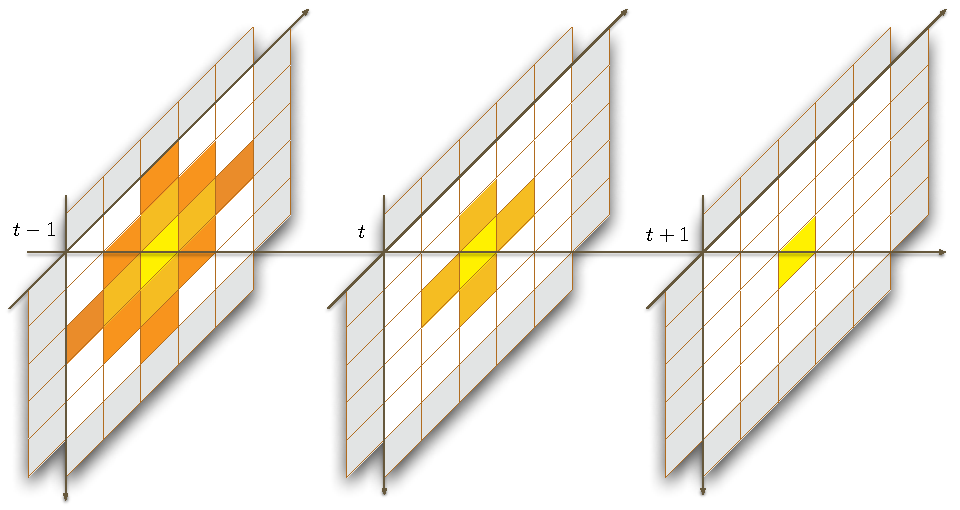
\includegraphics[scale=0.5]{figures/structured-updates.pdf}
  \end{figure} 
%
\end{frame}

% --------------------------------------
% numerics
\begin{frame}[fragile]
%
  \frametitle{Computing derivatives}
%
  \begin{itemize}
%
  \item there are three different first order approximations
    \begin{itemize}
%
    \item forward difference:
      \begin{equation}
      \partial \raisebox{-.4em}{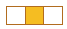
\includegraphics{figures/structured-1d-centered.pdf}}
      =
      \frac{1}{\delta}
      \left(
        \raisebox{-.4em}{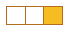
\includegraphics{figures/structured-1d-right.pdf}} 
        -
        \raisebox{-.4em}{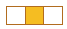
\includegraphics{figures/structured-1d-middle.pdf}} 
      \right)
      \end{equation}
%
    \item backward difference:
      \begin{equation}
      \partial \raisebox{-.4em}{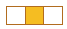
\includegraphics{figures/structured-1d-centered.pdf}}
      =
      \frac{1}{\delta}
      \left(
        \raisebox{-.4em}{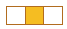
\includegraphics{figures/structured-1d-middle.pdf}} 
        -
        \raisebox{-.4em}{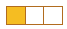
\includegraphics{figures/structured-1d-left.pdf}} 
      \right)
      \end{equation}
%
    \item central difference:
      \begin{equation}
      \partial \raisebox{-.4em}{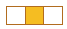
\includegraphics{figures/structured-1d-centered.pdf}}
      =
      \frac{1}{2\delta}
      \left(
        \raisebox{-.4em}{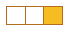
\includegraphics{figures/structured-1d-right.pdf}} 
        -
        \raisebox{-.4em}{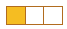
\includegraphics{figures/structured-1d-left.pdf}} 
      \right)
      \end{equation}
%
    \end{itemize}
    where $\delta$ is the uniform grid spacing
%
    \item forward and backward differences are most often used for {\em explicit} time
      integration
%
    \item central differences are used to compute spatial derivatives
%
    \item the second order central difference is given by
      \begin{equation}
      \partial \raisebox{-.2em}{
\includegraphics{figures/structured-1d-5c.pdf}}
      =
      \frac{1}{12\delta}
      \left(
        -
        \raisebox{-.2em}{
\includegraphics{figures/structured-1d-55.pdf}} 
        +
        8 \raisebox{-.2em}{
\includegraphics{figures/structured-1d-54.pdf}} 
        -
        8 \raisebox{-.2em}{
\includegraphics{figures/structured-1d-52.pdf}} 
        +
        \raisebox{-.2em}{
\includegraphics{figures/structured-1d-51.pdf}} 
      \right)
      \end{equation}
%
  \end{itemize}
%
\end{frame}

% --------------------------------------
% numerics
\begin{frame}[fragile]
%
  \frametitle{Partial derivatives in two dimensions}
%
  \begin{itemize}
%
  \item let $\delta_{x}$ and $\delta_{y}$ be the uniform grid spacing along each dimension
%
  \item then, the first order central difference approximations to the spatial derivatives are
    given by
    \begin{eqnarray}
      \partial_{x} \raisebox{-.5em}{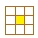
\includegraphics{figures/structured-2d-centered.pdf}}
      & = &
      \frac{1}{2\delta_{x}}
      \left(
        \raisebox{-.5em}{
\includegraphics{figures/structured-2d-e.pdf}} 
        - \raisebox{-.5em}{
\includegraphics{figures/structured-2d-w.pdf}} 
      \right )
      \\
      \partial_{y} \raisebox{-.5em}{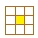
\includegraphics{figures/structured-2d-centered.pdf}}
      & = &
      \frac{1}{2\delta_{y}}
      \left(
        \raisebox{-.5em}{
\includegraphics{figures/structured-2d-s.pdf}} 
        - \raisebox{-.5em}{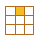
\includegraphics{figures/structured-2d-n.pdf}} 
      \right )
    \end{eqnarray}
%
  \item and the second order derivatives are given by
    \begin{eqnarray}
      \partial_{xx} \raisebox{-.5em}{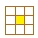
\includegraphics{figures/structured-2d-centered.pdf}}
      & = &
      \frac{1}{\delta_{x}^{2}}
      \left(
        \raisebox{-.5em}{
\includegraphics{figures/structured-2d-e.pdf}} 
        -2 \raisebox{-.5em}{
\includegraphics{figures/structured-2d-middle.pdf}} 
        + \raisebox{-.5em}{
\includegraphics{figures/structured-2d-w.pdf}} 
      \right )
      \\
      \partial_{yy} \raisebox{-.5em}{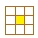
\includegraphics{figures/structured-2d-centered.pdf}}
      & = &
      \frac{1}{\delta_{y}^{2}}
      \left(
        \raisebox{-.5em}{
\includegraphics{figures/structured-2d-s.pdf}} 
        -2 \raisebox{-.5em}{
\includegraphics{figures/structured-2d-middle.pdf}} 
        + \raisebox{-.5em}{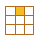
\includegraphics{figures/structured-2d-n.pdf}} 
      \right )
      \\
      \partial_{xy} \raisebox{-.5em}{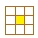
\includegraphics{figures/structured-2d-centered.pdf}}
      & = &
      \frac{1}{4\delta_{x}\delta_{y}}
      \left(
        \raisebox{-.5em}{
\includegraphics{figures/structured-2d-se.pdf}} 
        - \raisebox{-.5em}{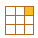
\includegraphics{figures/structured-2d-ne.pdf}} 
        - \raisebox{-.5em}{
\includegraphics{figures/structured-2d-sw.pdf}} 
        + \raisebox{-.5em}{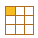
\includegraphics{figures/structured-2d-nw.pdf}} 
      \right )
    \end{eqnarray}
% 
  \end{itemize}
%
\end{frame}

% --------------------------------------
% example
\begin{frame}[fragile]
%
  \frametitle{Solving a simple PDE on a structured grid}
%
  \begin{itemize}
%
  \item Laplace's equation
    \begin{equation}
      \nabla^{2} \phi = 0
      \label{eq:laplace}
    \end{equation}
    over some domain $\Omega \in \mathbb{R}^{d}$, subject to Dirichlet boundary conditions
    \begin{equation}
      \phi(\partial \Omega) = f
    \end{equation}
%
  \item in two dimensions, using first order central differences, \eqref{laplace} becomes
    \begin{eqnarray}
      \raisebox{-.5em}{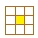
\includegraphics{figures/structured-2d-centered.pdf}}
      & = &
      \frac{1}{4}
      (
        \raisebox{-.5em}{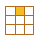
\includegraphics{figures/structured-2d-n.pdf}} 
        + \raisebox{-.5em}{
\includegraphics{figures/structured-2d-e.pdf}} 
        + \raisebox{-.5em}{
\includegraphics{figures/structured-2d-s.pdf}} 
        + \raisebox{-.5em}{
\includegraphics{figures/structured-2d-w.pdf}} 
      ) 
      \\
      & = &
      \frac{1}{4}
      \raisebox{-.5em}{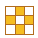
\includegraphics{figures/structured-2d-average.pdf}} 
      \label{eq:laplace-central}
    \end{eqnarray}
%
  \item we will solve this equation using the Jacobi iterative scheme:
    \begin{itemize}
    \item make an initial guess for $\phi$ over a discretization of $\Omega$
    \item apply the boundary conditions
    \item interpret \eqref{laplace-central} as an update step to compute the next iteration
      \begin{equation}
      \raisebox{-.5em}{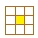
\includegraphics{figures/structured-2d-centered.pdf}}_{t+1}
      =
      \frac{1}{4}
      \raisebox{-.5em}{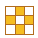
\includegraphics{figures/structured-2d-average.pdf}}_{t}
      \end{equation}
    \item stop when a convergence criterion is met
    \end{itemize}
% 
  \end{itemize}
%
\end{frame}

% --------------------------------------
% example
\begin{frame}[fragile]
%
  \frametitle{An example}
%
  \begin{itemize}
%
% 
  \item specifically,
    \begin{itemize}
    \item let $\Omega$ be the unit box in two dimensions
    \item and let $\phi$ satisfy the following boundary conditions
      \begin{equation}
        \begin{array}{rcrcll}
          & & \phi(x,0) & = & \sin(\pi x)           & 0 \leq x \leq 1 \\
          & & \phi(x,1) & = & \sin(\pi x) e^{-\pi}  & 0 \leq x \leq 1 \\
          \phi(0,y) & = & \phi(1, y) & = & 0        & 0 \leq y \leq 1
        \end{array}
      \end{equation}
    \end{itemize}
%
  \item the exact solution is given by
    \begin{equation}
      \phi(x,y) = \sin(\pi x) e^{-\pi y}
    \end{equation}
% 
  \end{itemize}
%
\end{frame}

% --------------------------------------
% parallelizing
\begin{frame}[fragile]
%
  \frametitle{Parallelization}
%
  \begin{itemize}
%
  \item with threads
  \item with \mpi
%
  \end{itemize}
% 
\end{frame}

% --------------------------------------
% threads
\begin{frame}[fragile]
%
  \frametitle{Parallelization with threads}
%
  \begin{itemize}
%
  \item
% 
  \end{itemize}
%
\end{frame}


% --------------------------------------
% partitioning
\begin{frame}[fragile]
%
  \frametitle{Partitioning the grid}
%
  \begin{itemize}
%
  \item {\em domain decomposition}
% 
  \end{itemize}
%
  \begin{figure}
    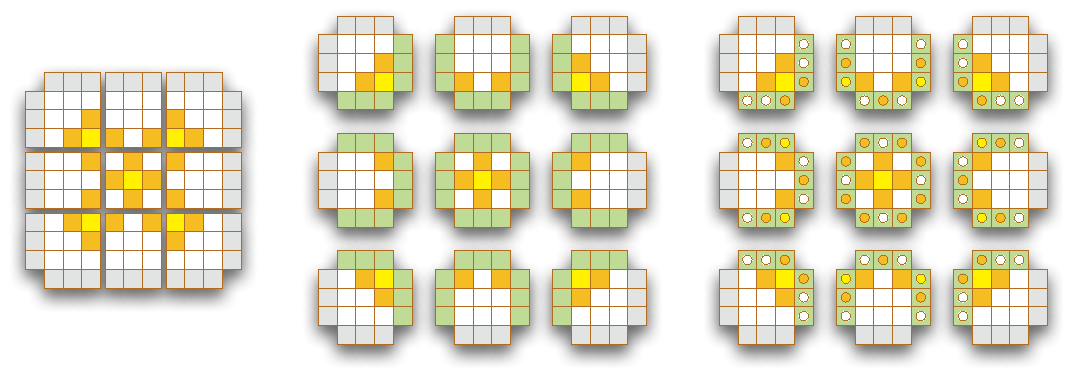
\includegraphics[scale=0.6]{figures/structured-partitioning.pdf}
  \end{figure} 
%
\end{frame}

% --------------------------------------
% communication patterns
\begin{frame}[fragile]
%
  \frametitle{Communication patterns}
%
  \begin{itemize}
%
  \item
% 
  \end{itemize}
%
\end{frame}

% --------------------------------------
% mpi virtual topologies
\begin{frame}[fragile]
%
  \frametitle{Using virtual topologies in \mpi}
%
  \begin{itemize}
%
  \item
% 
  \end{itemize}
%
\end{frame}

% --------------------------------------
% synchronous exchanges
\begin{frame}[fragile]
%
  \frametitle{Synchronous exchanges}
%
  \begin{itemize}
%
  \item
% 
  \end{itemize}
%
\end{frame}

% --------------------------------------
% asynchronous exchanges
\begin{frame}[fragile]
%
  \frametitle{Asynchronous exchanges}
%
  \begin{itemize}
%
  \item
% 
  \end{itemize}
%
\end{frame}


% end of file 
